%\documentclass[aps,prd,nofootinbib]{revtex4-1}
\documentclass[singlepage,notitlepage,nofootinbib,11pt]{revtex4-1}
\usepackage{amsmath}
\usepackage{graphicx}
\usepackage{subfig}
\usepackage{epsfig}
\usepackage{listings}
\usepackage[hidelinks,hyperfootnotes=false,bookmarks=false,colorlinks=true]{hyperref}

\newcommand{\eq}[1]{\begin{align*}#1\end{align*}}
\newcommand{\pmat}[1]{\begin{pmatrix}#1\end{pmatrix}}
\newcommand{\center}[1]{\begin{center}#1\end{center}}
\def\<{\langle}
\def\>{\rangle}
\def\l{\left}
\def\r{\right}


\begin{document}
\title{Problem Set 2 - G6080}
\author{Victor Genty}
\email{vgenty@nevis.columbia.edu}
\homepage{www.nevis.columbia.edu/~vgenty}
%\affiliation{Department of Physics, Duke University, Durham, NC 27707, USA}
\date{\today}
\begin{abstract}
\centering
Source code can be found at \href{https://github.com/vgenty/G6080/tree/master/ps3}{github.com/vgenty/G6080/ps3}
\end{abstract}
\maketitle
\section{Problem 1 - Stats of Mock Data}
\subsection{1.}
The true means for the 5 data sets for all 1,600,000 values are:
\begin{center}
\begin{tabular}{ | c | c | c | c | c |}\hline
  $\overline{v}_1$ &  $\overline{v}_2$ &  $\overline{v}_3$ &  $\overline{v}_4$ &  $\overline{v}_5$  \\ \hline \hline 
  1.76084 & 2.88634 & 4.01185 & 5.13712 & 6.26238 \\ \hline
\end{tabular}
\end{center}
\subsection{2.}
Histograms of sample means are shown in Fig. \ref{histos}. As the number of values in each sample increased, the standard deviation of the means is reduced by a factor of 
\eq{
\delta\sigma\approx\frac{1}{\sqrt{N}}\sim\frac{1}{\sqrt{10}},
}
as expected.
\begin{figure}[h]
  \centering
  \captionsetup[subfigure]{labelformat=empty}
  \subfloat[][]{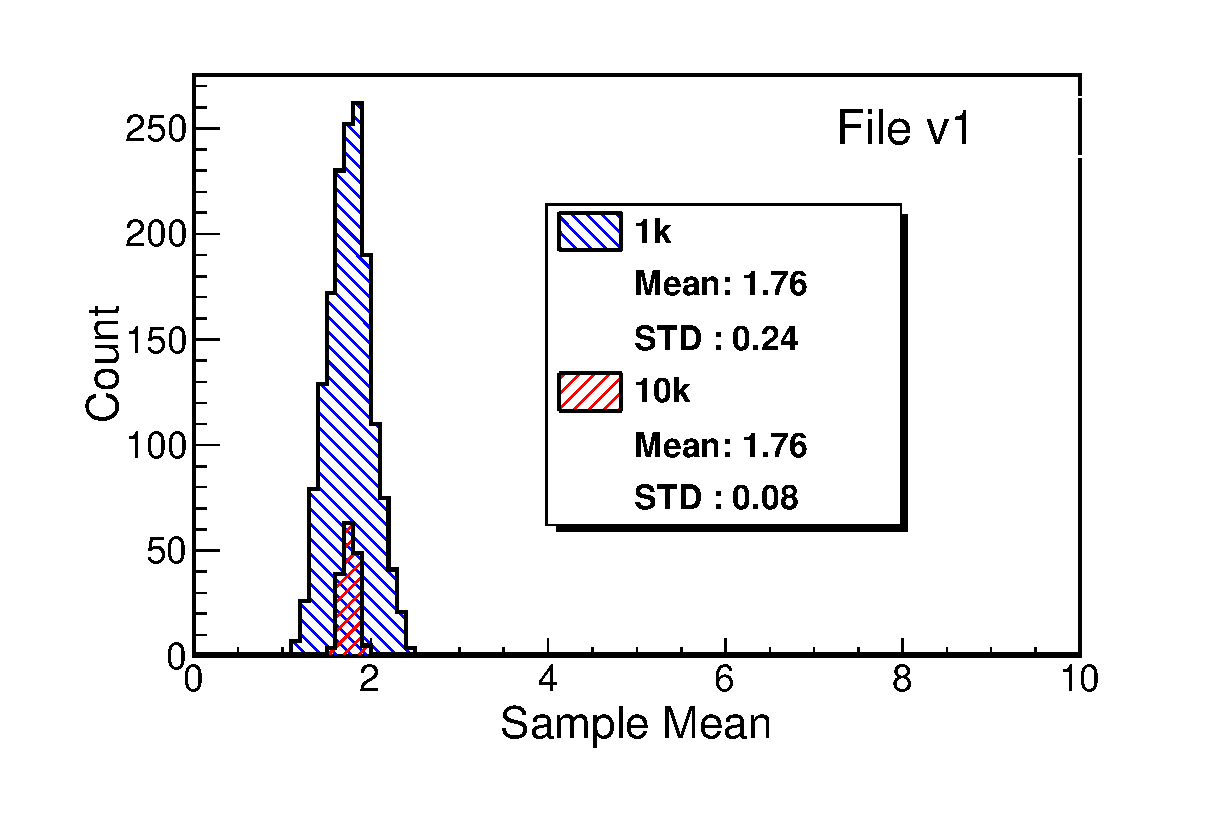
\includegraphics[width=0.5\textwidth]{figures/b1.eps}}
  \subfloat[][]{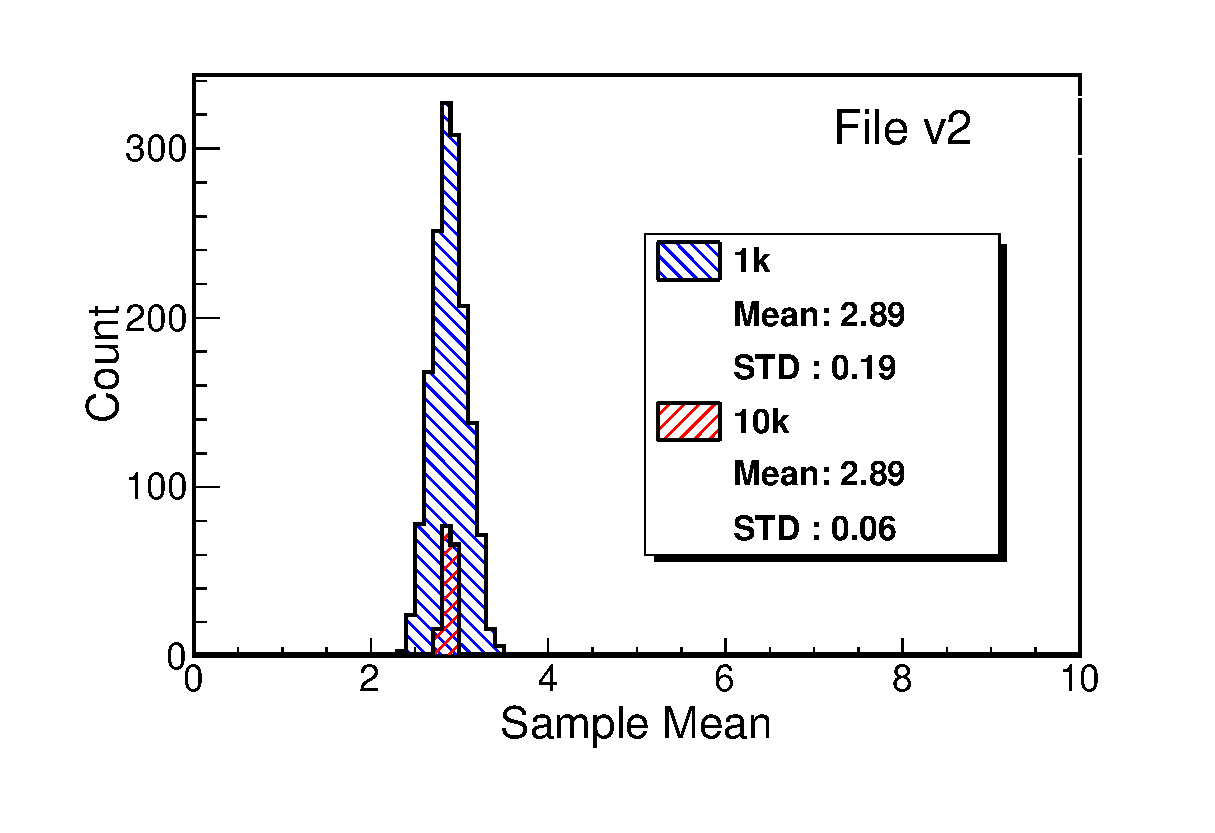
\includegraphics[width=0.5\textwidth]{figures/b2.eps}}\\
  \subfloat[][]{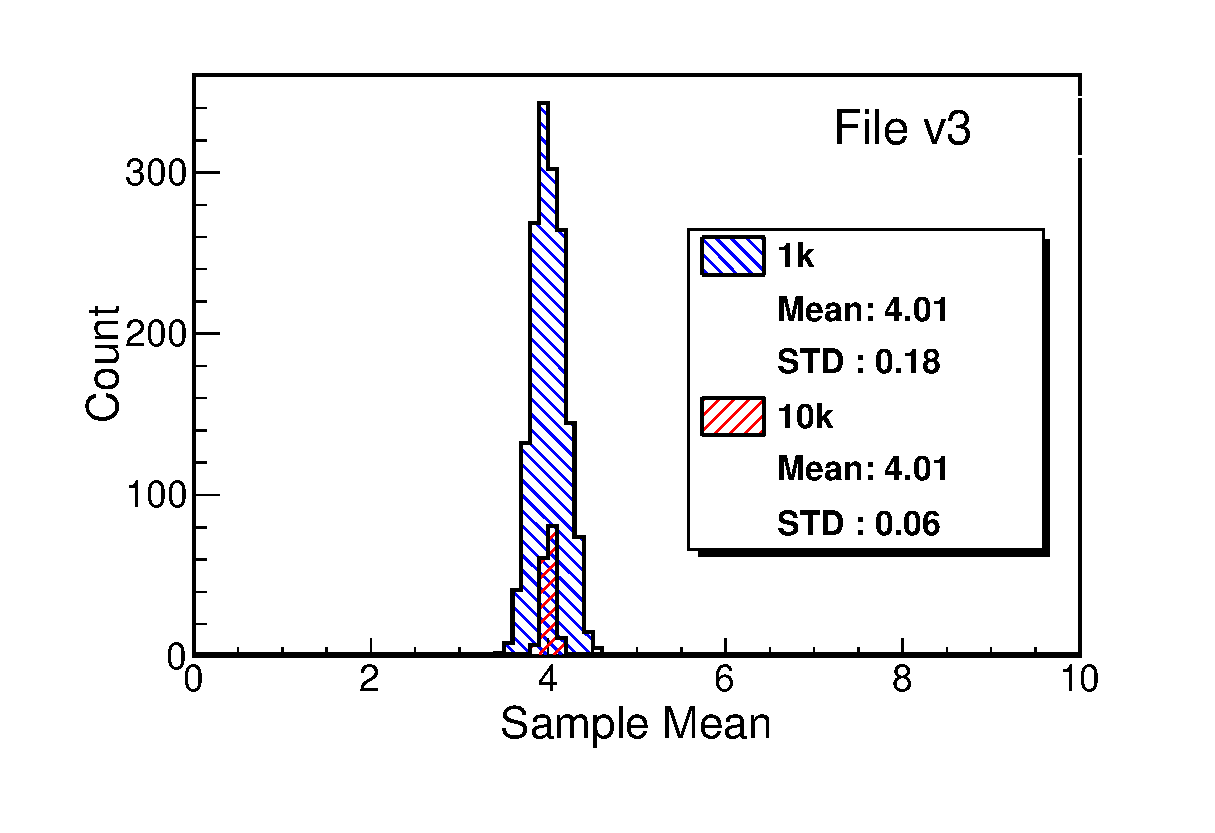
\includegraphics[width=0.5\textwidth]{figures/b3.eps}}
  \subfloat[][]{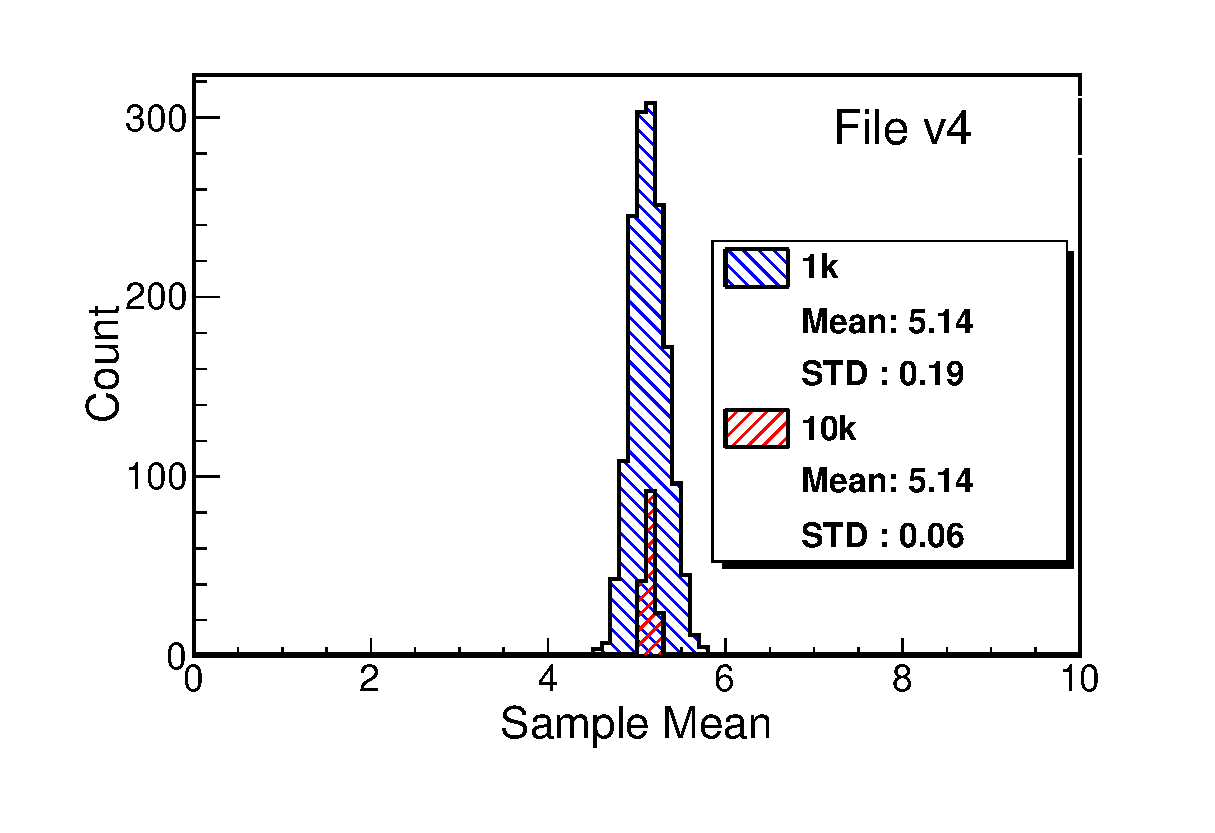
\includegraphics[width=0.5\textwidth]{figures/b4.eps}}\\
  \subfloat[][]{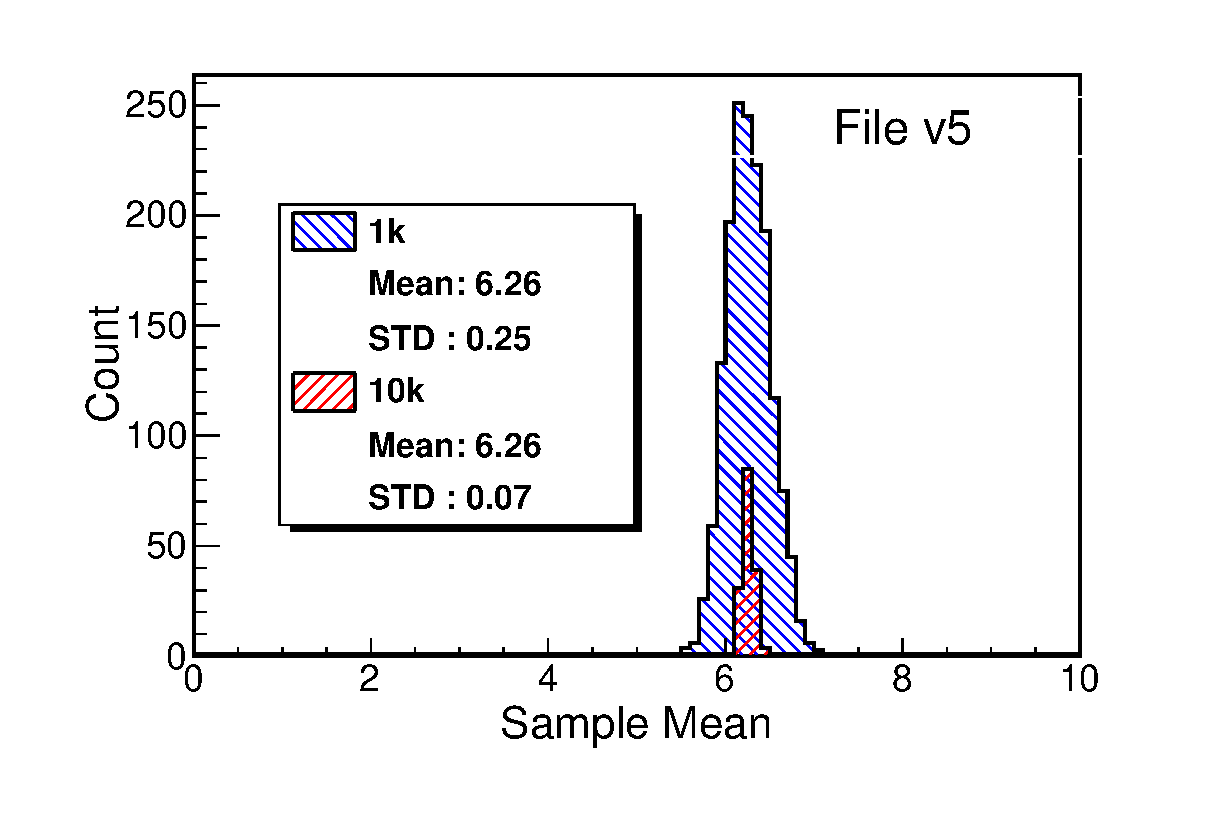
\includegraphics[width=0.5\textwidth]{figures/b5.eps}}
\hfill
  \caption{\label{histos} Histogram of sample means for 5 data sets. The blue shaded histogram contains the sample means for samples of size 1,000. The red histogram contains the sample means for samples of size 10,000. Increasing the number of sample means in each sample has the expected effect of narrowing the distribution.}
\end{figure}
\clearpage
\subsection{3}
We compute the true autocorrelation function for each of the data sets with the formula given in the problem. The normalized autocorrelation function $C_{v_a}(n)/C_{v_a}(0)$ for each data set is plotted versus $n_{\text{cut}}$ and shown in Fig. \ref{corrs}. The value of $n$ (or $n_{\text{cut}}$ which the auto-correlations disappear is roughly 100.
\begin{figure}[h]
  \centering
  \captionsetup[subfigure]{labelformat=empty}
  \subfloat[][]{\includegraphics[width=0.5\textwidth]{figures/c1.eps}}
  \subfloat[][]{\includegraphics[width=0.5\textwidth]{figures/c2.eps}}\\
  \subfloat[][]{\includegraphics[width=0.5\textwidth]{figures/c3.eps}}
  \subfloat[][]{\includegraphics[width=0.5\textwidth]{figures/c4.eps}}\\
  \subfloat[][]{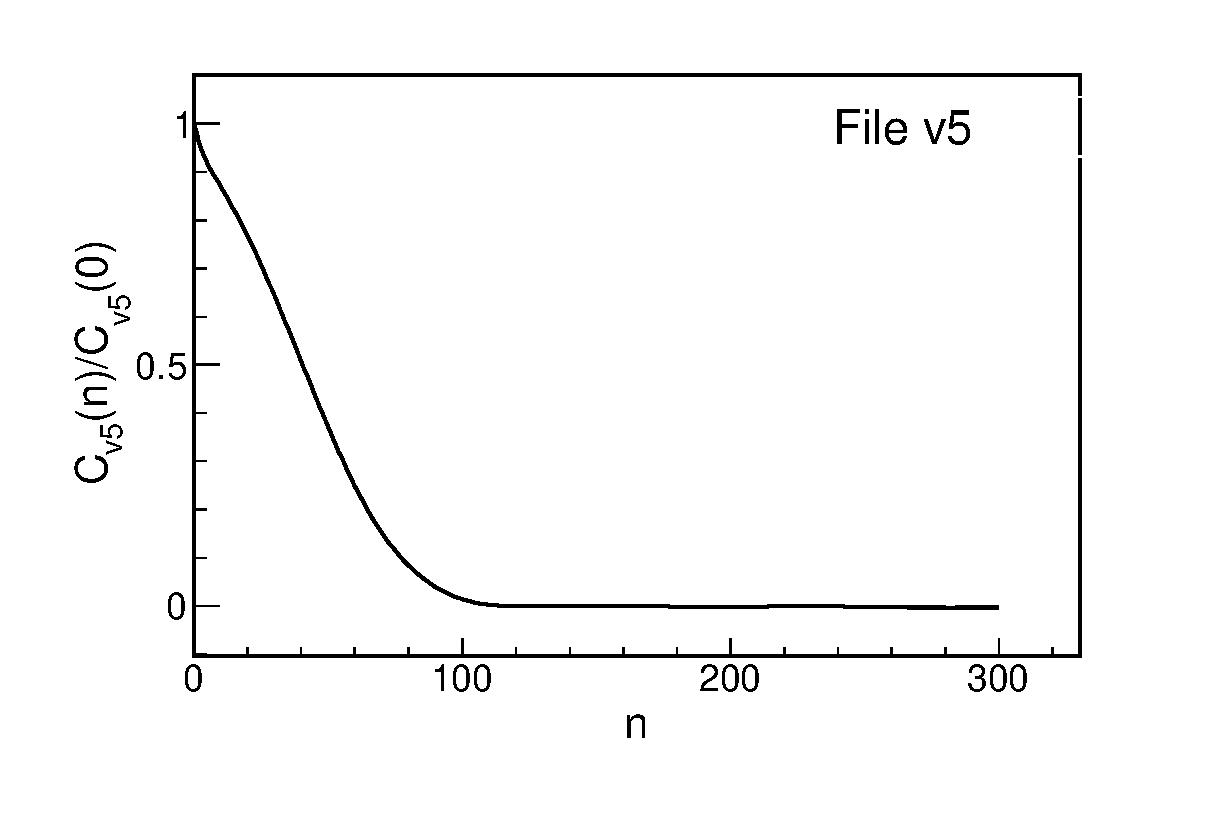
\includegraphics[width=0.5\textwidth]{figures/c5.eps}}
\hfill
  \caption{\label{corrs} Correlation functions for each of the data sets. It appears each set has auto-correlations on the order of 100 data points.}
\end{figure}
\clearpage
\subsection{4}
We estimate a value of $n_{\text{cut}}=125$. A small deviation in $n_{\text{cut}}$ around this value will not effect the integrated correlation time much. With this value we find the integrated correlation time for each of the data sets as,
\begin{center}
\begin{tabular}{ | c | c | c | c | c |}\hline
  $\tau_{\text{int},\overline{v}_1}$ &  $\tau_{\text{int},\overline{v}_2}$ &  $\tau_{\text{int},\overline{v}_3}$ &  $\tau_{\text{int},\overline{v}_4}$ &  $\tau_{\text{int},\overline{v}_5}$  \\ \hline \hline 
  41.73 & 42.38 & 40.03 & 42.77 & 49.02 \\ \hline
\end{tabular}
\end{center}
\section{Problem 2 - Jackknife of Mock Data}
\subsection{1}
One
\subsection{2}
Calculation of standard deviation from native propagation of errors...\\
$\mathbf{f_1}$
\eq{
\sigma_{f_1}^2 &= \l(\frac{\partial f_1}{\partial \overline{v}_1}\r)^2\sigma_{\overline{v}_1}^2 + \l(\frac{\partial f_1}{\partial \overline{v}_2}\r)^2\sigma_{\overline{v}_2}^2,\\
&=\l(\frac{1}{\overline{v}_2}\r)^2\sigma_{\overline{v}_1}^2 + \l(\frac{\overline{v}_1}{\overline{v}_2^2}\r)^2\sigma_{\overline{v}_2}^2,
}
so
\eq{
\boxed{\sigma_{f_1}=\sqrt{\l(\frac{1}{\overline{v}_2}\r)^2\sigma_{\overline{v}_1}^2 + \l(\frac{\overline{v}_1}{\overline{v}_2^2}\r)^2\sigma_{\overline{v}_2}^2}.}
}
$\mathbf{f_2}$
\eq{\sigma_{f_2}^2 &= \l(\frac{\partial f_2}{\partial \overline{v}_3}\r)^2\sigma_{\overline{v}_3}^2 + \l(\frac{\partial f_2}{\partial \overline{v}_4}\r)^2\sigma_{\overline{v}_4}^2,\\ 
  &=\exp\l(2(\overline{v}_3-\overline{v}_4)\r)\l(\sigma_{\overline{v}_3}^2+\sigma_{\overline{v}_4}^2\r),
}
so
\eq{
\boxed{ \sigma_{f_2} = \exp\l(\overline{v}_3-\overline{v}_4\r)\sqrt{\sigma_{\overline{v}_3}^2+\sigma_{\overline{v}_4}^2}}.
}
$\mathbf{f_3}$
\eq{
\sigma_{f_3}^2 &= \l(\frac{\partial f_3}{\partial \overline{v}_1}\r)^2\sigma_{\overline{v}_1}^2 + \l(\frac{\partial f_3}{\partial \overline{v}_2}\r)^2\sigma_{\overline{v}_2}^2 + \l(\frac{\partial f_3}{\partial \overline{v}_3}\r)^2\sigma_{\overline{v}_3}^2 + \l(\frac{\partial f_3}{\partial \overline{v}_4}\r)^2\sigma_{\overline{v}_4}^2 + \l(\frac{\partial f_3}{\partial \overline{v}_5}\r)^2\sigma_{\overline{v}_5}^2,
}
so
\eq{
\boxed{\sigma_{f_3} = \sqrt{\log^2(\overline{v}_5) \left(\frac{\overline{v}_1^2 \sigma_{\overline{v}_2}^2}{\overline{v}_2^4}+\frac{\sigma_{\overline{v}_1}^2}{\overline{v}_2^2}+\frac{\overline{v}_3^2 \sigma_{\overline{v}_4}^2}{\overline{v}_4^4}+\frac{\sigma_{\overline{v}_3}^2}{\overline{v}_4^2}\right)+\frac{\sigma_{\overline{v}_5}^2 (\overline{v}_1 \overline{v}_4+\overline{v}_2 \overline{v}_3)^2}{\overline{v}_2^2\,\overline{v}_4^2\,\overline{v}_5^2}}}
}
\end{document}
